% -*- LaTeX -*-
% -*- coding: utf-8 -*-
%
% michael a.g. aïvázis
% california institute of technology
% (c) 1998-2012 all rights reserved
%

\lecture{Structured grids}{20120215}

% --------------------------------------
% example
\begin{frame}[fragile]
%
  \frametitle{Solving a simple PDE on a uniform structured grid}
%
  \begin{itemize}
%
  \item Laplace equation over some domain $\Omega \in \mathbb{R}^{d}$, subject to Dirichlet
    boundary conditions
    \begin{equation}
      \begin{array}{ccc}
      \nabla^{2} \phi = 0 & {\rm with} & \phi(\partial \Omega) = f
      \end{array}
      \label{eq:laplace}
    \end{equation}
%
  \item let the grid be uniform: $\delta_{x} =  \delta_{y}$
%
  \item in two dimensions, using first order central differences, \eqref{laplace} becomes
    \begin{eqnarray}
      (\partial_{xx} + \partial_{yy})
      \raisebox{-.5em}{
\includegraphics{figures/structured-2d-middle.pdf}}
      & = &
      0
      \\
      4 \raisebox{-.5em}{
\includegraphics{figures/structured-2d-middle.pdf}} 
      & = &
      \raisebox{-.5em}{
\includegraphics{figures/structured-2d-e.pdf}} 
      + \raisebox{-.5em}{
\includegraphics{figures/structured-2d-w.pdf}} 
      + \raisebox{-.5em}{
\includegraphics{figures/structured-2d-s.pdf}} 
      + \raisebox{-.5em}{
\includegraphics{figures/structured-2d-n.pdf}} 
    \end{eqnarray}
%
  \item and translates into the following constraint among grid elements
    \begin{equation}
      \raisebox{-.5em}{
\includegraphics{figures/structured-2d-middle.pdf}}
      =
      \frac{1}{4}
      \raisebox{-.5em}{
\includegraphics{figures/structured-2d-average.pdf}} 
      \label{eq:laplace-central}
    \end{equation}
    using a shorthand for the sum of the neighboring cells
%
  \end{itemize}
%
\end{frame}

% --------------------------------------
% example
\begin{frame}[fragile]
%
  \frametitle{An example}
%
  \begin{itemize}
%
% 
  \item specifically,
    \begin{itemize}
    \item let $\Omega$ be the unit box in two dimensions
    \item and let $\phi$ satisfy the following boundary conditions
      \begin{equation}
        \begin{array}{rcrcll}
          & & \phi(x,0) & = & \sin(\pi x)           & 0 \leq x \leq 1 \\
          & & \phi(x,1) & = & e^{-\pi} \sin(\pi x)  & 0 \leq x \leq 1 \\
          \phi(0,y) & = & \phi(1, y) & = & 0        & 0 \leq y \leq 1
        \end{array}
      \end{equation}
    \end{itemize}
%
  \item the exact solution is given by
    \begin{equation}
      \phi(x,y) = e^{-\pi y} \sin(\pi x)
    \end{equation}
%
  \item we will solve this equation using the Jacobi iterative scheme:
    \begin{itemize}
    \item make an initial guess for $\phi$ over a discretization of $\Omega$
    \item apply the boundary conditions
    \item interpret \eqref{laplace-central} as an update step to compute the next iteration
      \begin{equation}
      \raisebox{-.5em}{
\includegraphics{figures/structured-2d-centered.pdf}}_{t}
      =
      \frac{1}{4}
      \raisebox{-.5em}{
\includegraphics{figures/structured-2d-average.pdf}}_{t-1}
      \end{equation}
    \item stop when a convergence criterion is met
    \end{itemize}
%
  \end{itemize}
%
\end{frame}

% --------------------------------------
% the solution
\begin{frame}[fragile]
%
  \frametitle{The solution}
%
  \begin{figure}
    \centering
    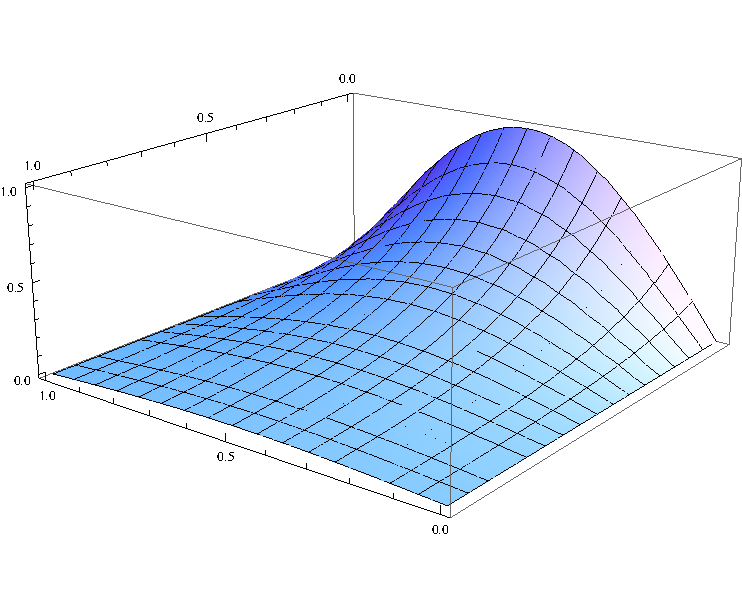
\includegraphics[width=0.9\linewidth]{figures/laplace-example.pdf}
    \label{fig:reduction-shared}
  \end{figure}
%
\end{frame}


% --------------------------------------
% parallelizing
\begin{frame}[fragile]
%
  \frametitle{Implementation strategy}
%
  \begin{itemize}
%
  \item grid resolution:
    \begin{itemize}
     \item ideally determined by analyzing the boundary conditions, since discrete sampling may
       wash out sharp features
     \item for our simple example, this can be done as part of the solver initialization
     \item we will use an $N \times N$ grid and let $N$ be user specified so we can control the
       problem size
       \begin{equation}
         \delta_{x} = \delta_{y} = \frac{1}{N-1}
       \end{equation}
     \end{itemize}
%
  \item data layout
    \begin{itemize}
    \item investigate the effect of data locality by trying out various layouts
    \end{itemize}
%
  \item setting up the update
    \begin{itemize}
      \item we only need to keep track of two iterants
      \item can be done in place; do you see how?
    \end{itemize}
%
  \item convergence criterion
    \begin{itemize}
    \item we will stop iterating when
      \begin{equation}
        \maximum{\Omega} (\phi_{t} - \phi_{t-1})) < \epsilon
      \end{equation}
      and let the user specify $\epsilon$
    \end{itemize}
%
  \end{itemize}
% 
\end{frame}

%
% \begin{figure}
%   \centering
%   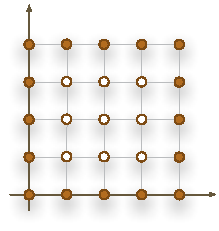
\includegraphics[scale=0.5]{figures/structured-dirichlet.pdf}
% \end{figure}

% --------------------------------------
% parallelization
\begin{frame}[fragile]
%
  \frametitle{Parallelization}
%
  \begin{itemize}
%
  \item the finest grain of work is clearly the cell update based on the value of its four
    nearest neighbors
%
  \item the shared memory implementation requires
    \begin{itemize}
    \item a scheme so that threads can update cells without the need for locks
    \item while maximizing locality of data access
    \item even the computation of the convergence criterion can be parallelized
    \end{itemize}
%
  \item with \mpi
    \begin{itemize}
    \item must partition the mesh among processes
    \item each process work on its own subgrid
    \item communication is required every iteration
    \item parallel convergence testing involves a collective operation
    \end{itemize}
%
  \end{itemize}
%
  \begin{figure}
    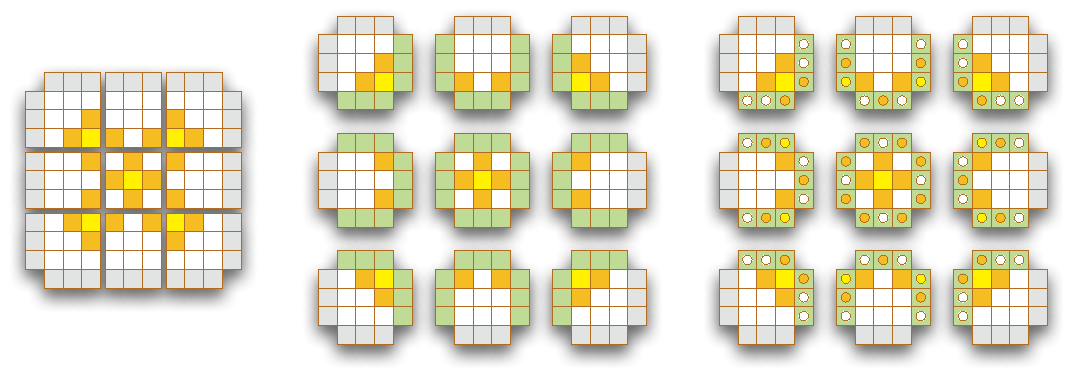
\includegraphics[scale=0.4]{figures/structured-partitioning.pdf}
  \end{figure} 
% 
\end{frame}

% --------------------------------------
% sequential
\begin{frame}[fragile]
%
  \frametitle{Sequential implementation - user interface}
%
  \begin{lstlisting}[language=c++,name=seq:frame,firstnumber=77]
// main program
int main(int argc, char* argv[]) {
    // default values for our user configurable settings
    size_t N = 10;
    double tolerance = 1.0e-6;
    const char* filename = "laplace.csv";

    // read the command line
    int command;
    while ((command = getopt(argc, argv, "N:e:o:")) != -1) {
        switch (command) {
        // get the convergence tolerance
        case 'e':
            tolerance = atof(optarg);
            break;
        // get the grid size
        case 'N':
            N = (size_t) atof(optarg);
            break;
        // get the name of the output file
        case 'o':
            filename = optarg;
        }
    }
    
  \end{lstlisting}
% 
\end{frame}

% --------------------------------------
% sequential
\begin{frame}[fragile]
%
  \frametitle{Sequential implementation - driving the solver}
%
  \begin{lstlisting}[language=c++,name=seq:frame]
    // allocate space for the solution
    Grid potential(N);

    // initialize and apply our boundary conditions
    initialize(potential);

    // call the solver
    laplace(potential, tolerance);

    // open a stream to hold the answer
    std::fstream output(filename, std::ios_base::out);

    // build a visualizer and render the solution in our chosen format
    Visualizer visualizer;
    visualizer.csv(potential, output);

    // all done
    return 0;
}
  \end{lstlisting}
% 
\end{frame}

% --------------------------------------
% sequential
\begin{frame}[fragile]
%
  \frametitle{Sequential implementation - user interface}
%
  \begin{lstlisting}[language=c++,name=seq:frame,firstnumber=77]
// main program
int main(int argc, char* argv[]) {
    // default values for our user configurable settings
    size_t N = 10;
    double tolerance = 1.0e-6;
    const char* filename = "laplace.csv";

    // read the command line
    int command;
    while ((command = getopt(argc, argv, "N:e:o:")) != -1) {
        switch (command) {
        // get the convergence tolerance
        case 'e':
            tolerance = atof(optarg);
            break;
        // get the grid size
        case 'N':
            N = (size_t) atof(optarg);
            break;
        // get the name of the output file
        case 'o':
            filename = optarg;
        }
    }
    
  \end{lstlisting}
% 
\end{frame}

% --------------------------------------
% sequential
\begin{frame}[fragile]
%
  \frametitle{Sequential implementation - driving the solver}
%
  \begin{lstlisting}[language=c++,name=seq:frame]
    // allocate space for the solution
    Grid potential(N);

    // initialize and apply our boundary conditions
    initialize(potential);

    // call the solver
    laplace(potential, tolerance);

    // open a stream to hold the answer
    std::fstream output(filename, std::ios_base::out);

    // build a visualizer and render the solution in our chosen format
    Visualizer visualizer;
    visualizer.csv(potential, output);

    // all done
    return 0;
}
  \end{lstlisting}
% 
\end{frame}

% --------------------------------------
% sequential
\begin{frame}[fragile]
%
  \frametitle{Sequential implementation - the preamble}
%
  \begin{itemize}
  \item back up to the beginning of the file
    \begin{lstlisting}[language=c++,name=seq:frame, firstnumber=1]
#include <getopt.h>
#include <cmath>
#include <cstdlib>
#include <fstream>
#include <iostream>

// forward declarations
class Grid;
class Visualizer;

// the solver; does nothing for the time being
void initialize(Grid & grid) {};
void laplace(Grid & grid, double tolerance){};

    \end{lstlisting}
%
  \item we have separated out {\em visualization} in a different object to support different
    formats without disturbing the data representation
%
  \item \identifier{initialize} and \identifier{laplace} have trivial implementations for now
    \begin{itemize}
    \item enables testing the scaffolding without worrying about the solver
      implementation just yet
    \end{itemize}
  \end{itemize}
% 
\end{frame}

% --------------------------------------
% sequential
\begin{frame}[fragile]
%
  \frametitle{Sequential implementation - the grid object stub}
%
  \begin{lstlisting}[language=c++,name=seq:frame]
// the solution representation
class Grid {
    // interface: TBD
public:

    // meta methods
public:
    Grid(size_t size);
    ~Grid();

    // private data members: TBD
private:

    // disabled interface
    // grid will own dynamic memory, so don't let the compiler screw up
private:
    Grid(const Grid &);
    const Grid & operator= (const Grid &);
};

// the grid implementation
Grid::Grid(size_t size) {
}

Grid::~Grid() {
}

  \end{lstlisting}
% 
\end{frame}

% --------------------------------------
% sequential
\begin{frame}[fragile]
%
  \frametitle{Sequential implementation - the visualizer stub}
%
  \begin{lstlisting}[language=c++,name=seq:frame, firstnumber=97]
// the visualizer class
class Visualizer {
    // local type aliases
public:
    typedef std::ostream stream_t;

    // interface
public:
    void csv(const Grid & grid, stream_t & stream);

    // meta methods
public:
    inline Visualizer() {}
};

// the Visualizer class implementation
void Visualizer::csv(const Grid & grid, Visualizer::stream_t & stream) {
    return;
}
  \end{lstlisting}
%

\begin{itemize}
\item the code now compiles and links
  \begin{itemize}
  \item consistency check that the object collaborations are ok, for now
  \item can be tested for command line option parsing
  \end{itemize}
\end{itemize}
% 
\end{frame}

% --------------------------------------
% the grid initializer
\begin{frame}[fragile]
%
  \frametitle{Fleshing out the initializer}
%
  \begin{lstlisting}[language=c++,name=seq:initializer]
// the grid initializer:
// clear the grid contents and apply our boundary conditions 
void initialize(Grid & grid) {
    // ask the grid to clear its memory
    grid.clear(1.0);
    // apply the dirichlet conditions
    for (size_t cell=0; cell < grid.size(); cell++) {
        // evaluate sin(pi x)
        double sin = std::sin(cell * grid.delta() * pi);
        // along the x axis, at top and  bottom
        grid(cell, 0) = sin;
        grid(cell, grid.size()-1) = sin * std::exp(-pi);
        // along the y axis, left and right
        grid(0, cell) = 0.0;
        grid(grid.size()-1, cell) = 0.0;
    }

    return;
}
  \end{lstlisting}
%
  \begin{itemize}
  \item the grid knows its size, its spacing $\delta$, and can initialize out its  memory
  \item access to grid elements happens through an overloaded \identifier{operator()} so we can
    {\em encapsulate} the indexing function
  \end{itemize}
%
\end{frame}

% --------------------------------------
% the grid declaration
\begin{frame}[fragile]
%
  \frametitle{The grid class declaration}
%
  \begin{lstlisting}[language=c++,name=seq:grid,firstnumber=29]
// the solution representation
class Grid {
    // interface
public:
    // set all cells to the specified value
    void clear(double value=0.0);
    // the grid dimensions
    size_t size() const {return _size;}
    // the grid spacing
    double delta() const {return _delta;}
    // access to the cells
    double & operator()(size_t i, size_t j) {return _block[j*_size+i];}
    double operator()(size_t i, size_t j) const {return _block[j*_size+i];}
    // meta methods
public:
    Grid(size_t size);
    ~Grid();
    // data members
private:
    const size_t _size;
    const double _delta;
    double* _block;
    // disable these
private:
    Grid(const Grid &);
    const Grid & operator= (const Grid &);
};

  \end{lstlisting}
%
\end{frame}

% --------------------------------------
% the grid implementation
\begin{frame}[fragile]
%
  \frametitle{The grid class implementation}
%
  \begin{lstlisting}[language=c++,name=seq:grid]
// the grid implementation
// interface
void Grid::clear(double value) {
    for (size_t i=0; i < _size*_size; i++) {
        _block[i] = value;
    }

    return;
}

// constructor
Grid::Grid(size_t size) :
    _size(size), 
    _delta((1.0 - 0.0)/(size-1)),
    _block(new double[size*size]) {
}

// destructor
Grid::~Grid() {
    delete [] _block;
}

  \end{lstlisting}
%
\end{frame}

% --------------------------------------
% the grid visualizer
\begin{frame}[fragile]
%
  \frametitle{Grid visualization}
%
  \begin{lstlisting}[language=c++,name=seq:visualizer,firstnumer=97]
// the visualizer class
class Visualizer {
    // local type aliases
public:
    typedef std::ostream stream_t;
    // interface
public:
    void csv(const Grid & grid, stream_t & stream);
    // meta methods
public:
    inline Visualizer() {}
};

// the Visualizer class implementation
void Visualizer::csv(const Grid & grid, Visualizer::stream_t & stream) {
    for (size_t j=0; j < grid.size(); j++) {
        stream << j;
        for (size_t i=0; i < grid.size(); i++) {
            stream << "," << grid(i,j);
        }
        stream << std::endl;
    }

    return;
}

  \end{lstlisting}
%
\end{frame}

% --------------------------------------
% the results of initialization
\begin{frame}[fragile]
%
  \frametitle{Printing out the initial grid}
%
  \begin{itemize}
  \item we should be able to print out the initialized grid
%
  \begin{shell}{}
#> mm laplace
#> laplace
#> cat laplace.csv
0,0,0.3827,0.7071,0.9239,1,0.9239,0.7071,0.3827,1.225e-16
1,0,1,1,1,1,1,1,1,0
2,0,1,1,1,1,1,1,1,0
3,0,1,1,1,1,1,1,1,0
4,0,1,1,1,1,1,1,1,0
5,0,1,1,1,1,1,1,1,0
6,0,1,1,1,1,1,1,1,0
7,0,1,1,1,1,1,1,1,0
8,0,0.01654,0.0306,0.03992,0.04321,0.0399,0.03056,0.01654,0
  \end{shell}
%
  \item notice that
    \begin{itemize}
    \item the top line contains some recognizable values
    \item the left and right borders are set to zero
    \item the interior of the grid is painted with our initial guess
    \end{itemize}
%
  \item still to do:
    \begin{itemize}
    \item write the update
    \item build a grid with the exact solution 
    \item build the error field (why?)
    \end{itemize}
  \end{itemize}
%
\end{frame}

% --------------------------------------
% the solver
\begin{frame}[fragile]
%
  \frametitle{Fleshing out the solver}
%
  \begin{lstlisting}[language=c++,basicstyle=\tt\bfseries\tiny,name=seq:solver,firstnumber=169]
// the solver driver
void laplace(Grid & current, double tolerance) {
    // create and initialize temporary storage
    Grid next(current.size());
    initialize(next);
    // put an upper bound on the number of iterations
    long max_iterations = (long) 1e4;;
    for (long iterations = 0; iterations<max_iterations; iterations++) {
        double max_dev = 0.0;
        // do an iteration step
        // leave the boundary alone
        // iterate over the interior of the grid
        for (size_t j=1; j < current.size()-1; j++) {
            for (size_t i=1; i < current.size()-1; i++) {
                // update
                next(i,j) = 0.25*(
                    current(i+1,j)+current(i-1,j)+current(i,j+1)+current(i,j-1));
                // compute the deviation from the last generation
                double dev = std::abs(next(i,j) - current(i,j));
                // and update the maximum deviation
                if (dev > max_dev) {
                    max_dev = dev;
                }
            }
        }
        // swap the blocks between the two grids
        Grid::swapBlocks(current, next);
        // check covergence
        if (max_dev < tolerance) {
            break;
        }
    }
    return;
}
  \end{lstlisting}
%
\end{frame}

% --------------------------------------
% the updated grid class
\begin{frame}[fragile]
%
  \frametitle{Adding the new grid interface}
%
  \begin{itemize}
  \item here is the declaration of \function{Grid::swapBlocks}
%
    \begin{lstlisting}[language=c++,firstnumber=30]
class Grid {
    // interface
    public:
    ...
    // exchange the data blocks of two compatible grids
    static void swapBlocks(Grid &, Grid &);
    ...
};
    \end{lstlisting}
%
  \item and its definition
%
    \begin{lstlisting}[language=c++,firstnumber=69]
void Grid::swapBlocks(Grid & g1, Grid & g2) {
    // bail out if the two operands are not compatible
    if (g1.size() != g2.size()) {
        throw "Grid::swapblocks: size mismatch";
    }
    if (g1.delta() != g2.delta()) {
        throw "Grid::swapblocks: spacing mismatch";
    }
    // but if they are, just exhange their data buffers
    double * temp = g1._block;
    g1._block = g2._block;
    g2._block = temp;
    // all done
    return;
}
    \end{lstlisting}
%
  \end{itemize}
%
\end{frame}

% --------------------------------------
% rework the driver to print out the exact solution and the error field
\begin{frame}[fragile]
%
  \frametitle{Reworking the driver}
%
  \begin{lstlisting}[language=c++,basicstyle=\tt\bfseries\tiny,name=seq:driver,firstnumber=239]
    // build a visualizer
    Visualizer vis;

    // compute the exact solution
    Grid solution(N);
    exact(solution);
    std::fstream exact_stream("exact.csv", std::ios_base::out);
    vis.csv(solution, exact_stream);
    
    // allocate space for the solution
    Grid potential(N);
    // initialize and apply our boundary conditions
    initialize(potential);
    // call the solver
    laplace(potential, tolerance);
    // open a stream to hold the answer
    std::fstream output_stream(filename, std::ios_base::out);
    // build a visualizer and render the solution in our chosen format
    vis.csv(potential, output_stream);

    // compute the error field
    Grid error(N);
    relative_error(potential, solution, error);
    std::fstream error_stream("error.csv", std::ios_base::out);
    vis.csv(error, error_stream);

    // all done
    return 0;
}
  \end{lstlisting}
%
\end{frame}

% --------------------------------------
% computing the exact and error fields
\begin{frame}[fragile]
% 
  \frametitle{Computing the exact solution and the error field}
%
  \begin{lstlisting}[language=c++,firstnumber=143]
void exact(Grid & grid) {
    //  paint the exact solution
    for (size_t j=0; j < grid.size(); j++) {
        for (size_t i=0; i < grid.size(); i++) {
            double x = i*grid.delta();
            double y = j*grid.delta();
            grid(i,j) = std::exp(-pi*y)*std::sin(pi*x);
        }
    }
    return;
}

void relative_error(
    const Grid & computed, const Grid & exact, Grid & error) {
    //  compute the relative error
    for (size_t j=0; j < exact.size(); j++) {
        for (size_t i=0; i < exact.size(); i++) {
            if (exact(i,j) == 0.0) { // hm... sloppy!
                error(i,j) = std::abs(computed(i,j));
            } else {
                error(i,j) = std::abs(computed(i,j) - exact(i,j))/exact(i,j);
            }
        }
    }
    return;
}

  \end{lstlisting}
%
\end{frame}

% --------------------------------------
% assessment
\begin{frame}[fragile]
%
  \frametitle{Shortcomings}
%
  \begin{itemize}
%
  \item numerics:
    \begin{itemize}
    \item it converges very slowly; other update {\em schemes} improve on this
    \item our approximation is very low order, so it takes very large grids to produce a few
      digits of accuracy
    \item the convergence criterion has some unwanted properties; it triggers
      \begin{itemize}
      \item prematurely: large swaths of constant values may never get updated
      \item it would trigger even if we were updating the wrong grid!
      \end{itemize}
    \end{itemize}
%
  \item design:
    \begin{itemize}
    \item separate the problem specification from its solution
    \item there are other objects lurking, waiting to be uncovered
    \item someone should make the graphic visualizer
    \item restarts anybody?
    \item how would you try out different convergence criteria? update schemes? memory layouts?
    \end{itemize}
%
    \item usability:
      \begin{itemize}
      \item supporting interchangeable parts requires damage to the top level driver
        \begin{itemize}
        \item to enable the user to make the selection
        \item to expose new command line arguments that configure the new parts
        \end{itemize}
      \end{itemize}
%
  \end{itemize}
%
\end{frame}

% --------------------------------------
% assessment
\begin{frame}[fragile]
%
  \frametitle{Assessing our fundamentals}
%
  \begin{itemize}
%
  \item \class{Grid} is a good starting point for abstracting structured grids
    \begin{itemize}
    \item assumes ownership of the memory associated with a structured grid
    \item encapsulates the indexing function
    \item extend it to
      \begin{itemize}
      \item support different memory layout strategies
      \item support non-square grids (?)
      \item support non-uniform grids (?)
      \item higher dimensions
      \item if you need any of these, consider using one of the many excellent class libraries
        written by experts
      \end{itemize}
    \end{itemize}
%
  \item \class{Visualizer}, under another name, can form the basis for a more general
    persistence library
    \begin{itemize}
    \item to support HDF5, NetCDF, bitmaps, voxels, etc.
    \end{itemize}
%
  \end{itemize}
%
\end{frame}

% --------------------------------------
% the Problem class
\begin{frame}[fragile]
% 
  \frametitle{The \class{Problem} class: the interface}
%
  \begin{lstlisting}[language=c++,name=Problem]
// the solution representation
class acm114::laplace::Problem {
    //typedefs
public:
    typedef std::string string_t;
    // interface
public:
    inline string_t name() const;
    inline const Grid & exact() const;
    inline const Grid & deviation() const;
    inline Grid & solution();
    inline const Grid & solution() const;
    inline Grid & error();
    inline const Grid & error() const;
    // abstract
    virtual void initialize() = 0;
    virtual void initialize(Grid &) const = 0;
    // meta methods
public:
    inline Problem(string_t name, double width, size_t points);
    virtual ~Problem();
    // data members
  \end{lstlisting}
%
\end{frame}

% --------------------------------------
% the Problem class
\begin{frame}[fragile]
% 
  \frametitle{The \class{Problem} class: the data}
%
  \begin{lstlisting}[language=c++,name=Problem]
protected:
    string_t _name;
    double _delta;
    Grid _solution;
    Grid _exact;
    Grid _error;
    Grid _deviation;
    // disable these
private:
    Problem(const Problem &);
    const Problem & operator= (const Problem &);
};
  \end{lstlisting}
%
\end{frame}

% --------------------------------------
% our specific example
\begin{frame}[fragile]
% 
  \frametitle{The \class{Example} class}
%
  \begin{lstlisting}[language=c++]
class acm114::laplace::Example : public acm114::laplace::Problem {
    // interface
public:
    virtual void initialize();
    virtual void initialize(Grid &) const;

    // meta methods
public:
    inline Example(string_t name, double width, size_t points);
    virtual ~Example();

    // disable these
private:
    Example(const Example &);
    const Example & operator= (const Example &);
};

  \end{lstlisting}
%
\end{frame}

% --------------------------------------
% the solver basis
\begin{frame}[fragile]
% 
  \frametitle{The \class{Solver} class}
%
  \begin{lstlisting}[language=c++]
class acm114::laplace::Solver {
    // interface
public:
    virtual void solve(Problem &) = 0;

    // meta methods
public:
    inline Solver();
    virtual ~Solver();

    // data members
private:

    // disable these
private:
    Solver(const Solver &);
    const Solver & operator= (const Solver &);
};

  \end{lstlisting}
%
\end{frame}

% --------------------------------------
% the jacobi solver 
\begin{frame}[fragile]
% 
  \frametitle{The \class{Jacobi} class}
%
  \begin{lstlisting}[language=c++]
class acm114::laplace::Jacobi : public acm114::laplace::Solver {
    // interface
public:
    virtual void solve(Problem &);

    // meta methods
public:
    inline Jacobi(double tolerance, size_t workers);
    virtual ~Jacobi();

    // implementation details
protected:
    virtual void _solve(Problem &);
    static void * _update(void *);

    // data members
private:
    double _tolerance;
    size_t _workers;

    // disable these
private:
    Jacobi(const Jacobi &);
    const Jacobi & operator= (const Jacobi &);
};

  \end{lstlisting}
%
\end{frame}

% --------------------------------------
% parallelization using threads
\begin{frame}[fragile]
%
  \frametitle{Parallelization using threads}
%
  \begin{itemize}
%
  \item the shared memory implementation requires
    \begin{itemize}
    \item a scheme so that threads can update cells without the need for locks
    \item while maximizing locality of data access
    \item even the computation of the convergence criterion can be parallelized
    \end{itemize}
%
  \item parallelization strategy
    \begin{itemize}
    \item we will focus on parallelizing the iterative grid update
      \begin{itemize}
      \item grid initialization, visualization, computing the exact answer and the error field
        do not depend on the {\em number of iterations}
      \end{itemize}
    \item the finest grain of work is clearly an individual cell update based on the value of
      its four nearest neighbors
    \item for this two dimensional example, we can build coarser grain tasks using
      \begin{itemize}
      \item horizontal or vertical strips
      \item non-overlapping blocks
      \item the strategy gets more complicated if you want to perform the update in place
      \end{itemize}
    \item the communication patterns are trivial for the double buffering layout; only the
      final update of the convergence criterion requires any locking
    \item each coarse grain task can be assigned to a thread
    \end{itemize}
%
  \end{itemize}
% 
\end{frame}

% --------------------------------------
% required changes to the sequential driver
\begin{frame}[fragile]
%
  \frametitle{Required changes to the sequential solution}
%
  \begin{itemize}
%
  \item what is needed
    \begin{itemize}
    \item an object to hold the problem information shared among the threads
    \item the per-thread administrative data structure that holds the thread id and the pointer
      to the shared information
      \begin{itemize}
      \item this is the argument to \function{pthread\_create}
      \end{itemize}
    \item a mutex to protect the update of the global convergence criterion
    \item a \function{pthread\_create} compatible worker routine
    \item a change at the top-level driver to enable the user to choose the number of threads
    \end{itemize}
%
  \item and a strategy for managing the thread life cycle
    \begin{itemize}
%
    \item synchronization is trivial if
      \begin{itemize}
      \item we spawn our threads to perform the updates of a single iteration
      \item harvest them
      \item check the convergence criterion 
      \item stop, or respawn them if another iteration is necessary
      \end{itemize}
%
    \item can the convergence test be done in parallel?
      \begin{itemize}
        \item so we don't have to pay the create/harvest overhead?
        \item if so, how do we guarantee correctness and consistency?
      \end{itemize}
%
    \end{itemize}
% 
  \end{itemize}
%
\end{frame}

% --------------------------------------
% the jacobi solver 
\begin{frame}[fragile]
% 
  \frametitle{Threaded \class{Jacobi}: thread data}
%
  \begin{lstlisting}[language=c++,name=Jacobi:threaded]
struct Task {
    // shared information 
    size_t workers;
    Grid & current;
    Grid & next;
    double maxDeviation;
    // mutex to control access to the convergence criterion
    pthread_mutex_t lock; 

    // constructor
    Task(size_t workers, Grid & current, Grid & next) :
        workers(workers), current(current), next(next), maxDeviation(0.0) {
        pthread_mutex_init(&lock, 0);
    }
    // destructor
    ~Task() {
        pthread_mutex_destroy(&lock);
    }
};

struct Context {
    // thread info
    size_t id;
    pthread_t descriptor;
    Task * task;
};

  \end{lstlisting}
%
\end{frame}

% --------------------------------------
% the jacobi solver 
\begin{frame}[fragile]
% 
  \frametitle{Threaded \class{Jacobi}: driving the update}
%
  \begin{lstlisting}[language=c++,name=Jacobi:threaded]
void Jacobi::solve(Problem & problem) {
    // initialize the problem
    problem.initialize();
    // do the actual solve
    _solve(problem);
    // compute and store the error
    std::cout << "  computing absolute error" << std::endl;
    //  compute the relative error
    Grid & error = problem.error();
    const Grid & exact = problem.exact();
    const Grid & solution = problem.solution();

    for (size_t j=0; j < exact.size(); j++) {
        for (size_t i=0; i < exact.size(); i++) {
            if (exact(i,j) == 0.0) {
                error(i,j) = std::abs(solution(i,j));
            } else {
                error(i,j) = std::abs(solution(i,j) - exact(i,j))/exact(i,j);
            }
        }
    }
    std::cout << " --- done." << std::endl;
    return;
}
  \end{lstlisting}
%
\end{frame}

% --------------------------------------
% the jacobi solver 
\begin{frame}[fragile]
% 
  \frametitle{Threaded \class{Jacobi}: the master thread}
%
  \begin{lstlisting}[language=c++,name=Jacobi:threaded]
void Jacobi::_solve(Problem & problem) {
    Grid & current = problem.solution();

    // create and initialize temporary storage
    Grid next(current.size());
    problem.initialize(next);

    // shared thread info
    Task task(_workers, current, next);
    // per-thread information
    Context context[_workers];

    // let's get going
    std::cout << "jacobi: tolerance=" << _tolerance << std::endl;

    // put an upper bound on the number of iterations
    const size_t max_iterations = (size_t) 1.0e4;
  \end{lstlisting}
%
\end{frame}

% --------------------------------------
% the jacobi solver 
\begin{frame}[fragile]
% 
  \frametitle{Threaded \class{Jacobi}: the master thread, part 2}
%
  \begin{lstlisting}[language=c++,name=Jacobi:threaded,basicstyle=\tt\bfseries\tiny]
    for (size_t iterations = 0; iterations<max_iterations; iterations++) {
        if (iterations % 100 == 0) {
            std::cout << "     " << iterations << std::endl;
        }
        // reset the maximium deviation
        task.maxDeviation = 0.0;
        // spawn the threads
        for (size_t tid=0; tid < _workers; tid++) {
            context[tid].id = tid;
            context[tid].task = &task;

            int status = pthread_create(&context[tid].descriptor, 0, _update, &context[tid]);
            if (status) {
                throw ("error in pthread_create");
            }
        }
        // harvest the threads
        for (size_t tid = 0; tid < _workers; tid++) {
            pthread_join(context[tid].descriptor, 0);
        }

        // swap the blocks between the two grids
        Grid::swapBlocks(current, next);
        // check covergence
        if (task.maxDeviation < _tolerance) {
            std::cout << " ### convergence in " << iterations << " iterations!" << std::endl;
            break;
        }
    }
    std::cout << " --- done." << std::endl;

    return;
}
  \end{lstlisting}
%
\end{frame}

% --------------------------------------
% the jacobi solver 
\begin{frame}[fragile]
% 
  \frametitle{Threaded \class{Jacobi}: update in the worker threads}
%
  \begin{lstlisting}[language=c++,basicstyle=\tt\bfseries\tiny,name=Jacobi:threaded]
void * Jacobi::_update(void * arg) {
    Context * context = static_cast<Context *>(arg);

    size_t id = context->id;
    Task * task = context->task;

    size_t workers = task->workers;
    Grid & current = task->current;
    Grid & next = task->next;
    pthread_mutex_t lock = task->lock;

    double max_dev = 0.0;
    // do an iteration step
    // leave the boundary alone
    // iterate over the interior of the grid
    for (size_t j=id+1; j < current.size()-1; j+=workers) {
        for (size_t i=1; i < current.size()-1; i++) {
            next(i,j) = 0.25*(current(i+1,j)+current(i-1,j)+current(i,j+1)+current(i,j-1));
            // compute the deviation from the last generation
            double dev = std::abs(next(i,j) - current(i,j));
            // and update the maximum deviation
            if (dev > max_dev) {
                max_dev = dev;
            }
        }
    }

    // grab the lock and update the global maximum deviation
    pthread_mutex_lock(&lock);
    if (task->maxDeviation < max_dev) {
        task->maxDeviation = max_dev;
    }
    pthread_mutex_unlock(&lock);

    return 0;
}
  \end{lstlisting}
%
\end{frame}

% --------------------------------------
% improving the threaded implementation
\begin{frame}[fragile]
%
  \frametitle{Assessing the threaded implementation}
%
  \begin{itemize}
%
  \item the implemented synchronization scheme is very simple
    \begin{itemize}
    \item each grid update step spawns some number of workers to update a subset of the cells
    \item the workers are harvested after the grid is updated
    \item the main thread checks for convergence
    \item if another iteration is required, a new set of workers is spawned
    \end{itemize}
%
  \item the simplicity of this strategy comes at a cost
    \begin{itemize}
    \item {\em scalability} suffers when the overhead of creating and harvesting threads is
      comparable to amount of work done by each thread
    \item for low thread counts, it is still an overall win, since the time to solution
      decreases and the machine utilization is better
    \item but as the number of threads increases, the program becomes {\em slower}
      \begin{itemize}
      \item timing a $100\times100$ grid to convergence on a recent MacPro
%
        \begin{equation*}
          \begin{array}{r|ccccc}
% header
            {\rm threads } & 1 & 2 & 4 & 8 & 16 \\
            \hline 
            {\rm time} (s) & 4.367 & 2.517 & 1.918 & 1.937 & 3.537
% 
          \end{array}
        \end{equation*}
      \item and 10,000 iterations of a $1000\times1000$ grid
        \begin{equation*}
          \begin{array}{r|ccccc}
% header
            {\rm threads } & 1 & 2 & 4 & 8 & 16 \\
            \hline 
            {\rm time} (s) & 413.306 & 211.050 & 109.509 & 98.279 & 74.087
% 
          \end{array}
        \end{equation*}
      \end{itemize}

    \end{itemize}
%
\end{itemize}
%
\end{frame}

% --------------------------------------
% Improving the update loop
\begin{frame}[fragile]
%
  \frametitle{Improving the update loop}
%
  \begin{itemize}
%
  \item the plan is to keep the workers alive and updating the grid while either we converge or
    \identifier{max\_iterations} is reached
  \item the main thread
    \begin{itemize}
    \item loops to spawn all the threads
    \item and immediately enters a loop to harvest them
    \end{itemize}
%
  \item the workers use a condition variable to synchronize among themselves
    \begin{itemize}
    \item they iterate, updating the grid
    \item grab a mutex, deposit their local maximum deviation from the last iterations, update
      a counter that records how many workers have completed their update, and release the lock
    \item enter another critical section with the termination logic
      \begin{itemize}
      \item everybody uses a condition variable to wait for the slowest worker
      \item the slowest worker checks the convergence criterion and updates the termination
        flag, swaps the grid blocks and signals everybody else
      \item if the termination flag is set, or if the maximum number of iterations has been
        reached, all threads exit
      \end{itemize}
    \end{itemize}
%
  \end{itemize}
%
\end{frame}

% --------------------------------------
% the jacobi solver 
\begin{frame}[fragile]
% 
  \frametitle{Threaded \class{Jacobi}: the main thread}
%
  \begin{lstlisting}[language=c++,name=Jacobi:updated-solve,basicstyle=\tt\bfseries\tiny]
void Jacobi::_solve(Problem & problem) {
    Grid & current = problem.solution();

    // create and initialize temporary storage
    Grid next(current.size());
    problem.initialize(next);

    // shared thread info
    Task task(_workers, _tolerance, current, next);
    // per-thread information
    Context context[_workers];
    // spawn the threads
    std::cout << "jacobi: spawning " << _workers << " workers" << std::endl;
    for (size_t tid=0; tid < _workers; tid++) {
        context[tid].id = tid;
        context[tid].task = &task;
        
        int status = pthread_create(&context[tid].descriptor, 0, _update, &context[tid]);
        if (status) {
            throw ("error in pthread_create");
        }
    }
    // harvest the threads
    for (size_t tid = 0; tid < _workers; tid++) {
            pthread_join(context[tid].descriptor, 0);
        }
    // done
    std::cout << "jacobi: done." << std::endl;
    return;
}
  \end{lstlisting}
%
\end{frame}

% --------------------------------------
% the jacobi solver 
\begin{frame}[fragile]
% 
  \frametitle{Threaded \class{Jacobi}: updated thread data}
%
  \begin{lstlisting}[language=c++,name=Jacobi:updated-threaded,basicstyle=\tt\bfseries\tiny]
struct Task {
    // shared information 
    size_t workers; // the number of threads
    double tolerance; // the covergence tolerance
    Grid & current;
    Grid & next;

    bool done; // is there more work?
    double maxDeviation; // the value
    size_t contributions; // the number of threads that have deposited contributions
    pthread_mutex_t gridUpdate_lock; //the mutex
    pthread_cond_t gridUpdate_check;

    Task(size_t workers, double tolerance, Grid & current, Grid & next) :
        workers(workers), tolerance(tolerance), current(current), next(next),
        done(false), maxDeviation(0.0), contributions(0),
        gridUpdate_lock(), gridUpdate_check() {
        // initialize the grid update lock
        pthread_mutex_init(&gridUpdate_lock, 0);
        pthread_cond_init(&gridUpdate_check, 0);
    }

    ~Task() {
        pthread_mutex_destroy(&gridUpdate_lock);
        pthread_cond_destroy(&gridUpdate_check);
    }
};

  \end{lstlisting}
%
\end{frame}

% --------------------------------------
% the jacobi solver 
\begin{frame}[fragile]
% 
  \frametitle{Threaded \class{Jacobi}: workers, part 1}
%
  \begin{lstlisting}[language=c++,name=Jacobi:updated-solve,basicstyle=\tt\bfseries\tiny]
// the threaded update
void * Jacobi::_update(void * arg) {
    Context * context = static_cast<Context *>(arg);

    size_t id = context->id;
    Task * task = context->task;

    const size_t workers = task->workers;
    Grid & current = task->current;
    Grid & next = task->next;

    size_t maxIterations = (size_t) 1e4;
    // iterate, updating the grid until done
    for (size_t iteration = 0; iteration < maxIterations; iteration++) {
        // thread 0: print an update
        if (id == 0 && iteration % 100 == 0) {
            std::cout << "    " << iteration << std::endl;
        }

        double max_dev = 0.0;
        // do an iteration step
        // leave the boundary alone
        // iterate over the interior of the grid
        for (size_t j=id+1; j < current.size()-1; j+=workers) {
            for (size_t i=1; i < current.size()-1; i++) {
                next(i,j) = 0.25*(current(i+1,j)+current(i-1,j)+current(i,j+1)+current(i,j-1));
                // compute the deviation from the last generation
                double dev = std::abs(next(i,j) - current(i,j));
                // and update the maximum deviation
                if (dev > max_dev) {
                    max_dev = dev;
                }
            }
        }
        // done with the grid update
  \end{lstlisting}
%
\end{frame}

% --------------------------------------
% the jacobi solver 
\begin{frame}[fragile]
% 
  \frametitle{Threaded \class{Jacobi}: workers, part 2}
%
  \begin{lstlisting}[language=c++,name=Jacobi:updated-solve,basicstyle=\tt\bfseries\tiny]
        // grab the grid update lock
        pthread_mutex_lock(&task->gridUpdate_lock);
        // update the global maximum deviation 
        if (task->maxDeviation < max_dev) {
            task->maxDeviation = max_dev;
        }
        // leave a mark
        task->contributions++;
        // bookkeeping at the end of the  update
        if (task->contributions == workers) {
            // if i am the slowest worker
            // swap the blocks between the two grids
            Grid::swapBlocks(current, next);
            // check covergence
            if (task->maxDeviation < task->tolerance) {
                std::cout
                    << " +++ thread " << id << ": convergence in " << iteration << " iterations"
                    <<std::endl;
                task->done = true;
            }
            // reset our accounting and signal everybody
            task->contributions = 0;
            task->maxDeviation = 0;
            pthread_cond_broadcast(&task->gridUpdate_check);
        } else {
            // all but the slowest wait here
            pthread_cond_wait(&task->gridUpdate_check, &task->gridUpdate_lock);
        } 
        // release
        pthread_mutex_unlock(&task->gridUpdate_lock);
        // check whether we are done
        if (task->done) {
            break;
        }
    }
    return 0;
}
  \end{lstlisting}
%
\end{frame}

% --------------------------------------
% improving the threaded implementation
\begin{frame}[fragile]
%
  \frametitle{Assessing the improved implementation}
%
  \begin{itemize}
%
  \item the improved threading scheme is not much more complex
    \begin{itemize}
    \item we keep track of how many threads have computed their grid update
    \item the slowest worker check the convergence criterion and performs all the necessary
      bookkeeping 
    \item while everybody else waits
    \item use \function{pthread\_cond\_brodacast} to wake the other workers
    \end{itemize}
%
  \item here is the performance comparison for 10,000 iterations on a $1000 \times 1000$ grid
    on the same 8-core MacPro
    \begin{equation*}
      \begin{array}{r|ccccc}
% header
        {\rm threads } & 1 & 2 & 4 & 8 & 16 \\
        \hline 
        {\rm previous} (s) & 413.306 & 211.050 & 109.509 & 98.279 & 74.087 \\
        {\rm updated} (s)  & 408.636 & 208.832 & 107.015 & 59.043 & 61.481 \\
% 
      \end{array}
    \end{equation*}
%
  \end{itemize}
%
\end{frame}

% --------------------------------------
% parallelization with MPI
\begin{frame}[fragile]
%
  \frametitle{Parallelization with \mpi}
%
  \begin{itemize}
%
  \item the \mpi\ implementation will require careful data management
    \begin{itemize}
    \item we must partition the mesh among processes
    \item each process work on its own subgrid
      \begin{itemize}
      \item it will allocate its own memory, for both actual data and the guard zones
      \item it must locate its patch in physical space
      \end{itemize}
    \item communication is required every iteration
      \begin{itemize}
      \item so that neighbors can synchronize their boundaries
      \item think of the synchronization as a kind of boundary condition!
      \end{itemize}
    \item parallel convergence testing involves a collective operation
    \end{itemize}
%
  \end{itemize}
%
  \begin{figure}
    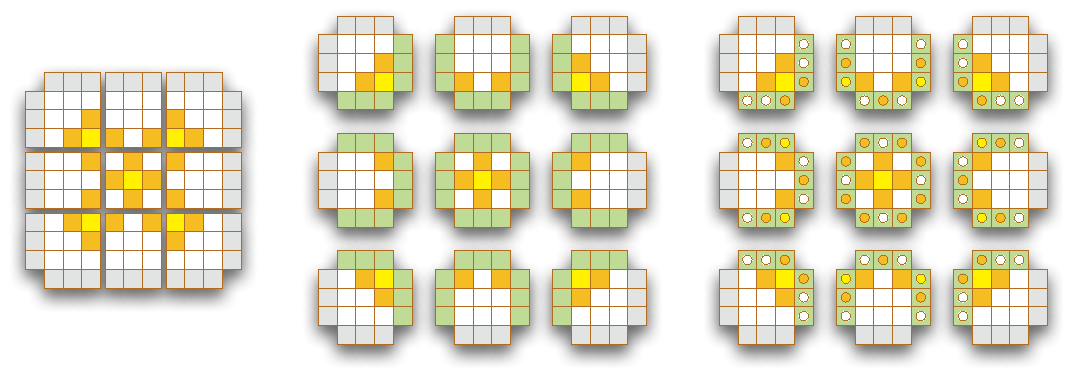
\includegraphics[scale=0.5]{figures/structured-partitioning.pdf}
  \end{figure} 
% 
\end{frame}

% --------------------------------------
% template
\begin{frame}[fragile]
%
  \frametitle{A little bit of help}
%
  \begin{itemize}
%
  \item \mpi\ supports this common use case through a Cartesian {\em virtual topology}
    \begin{itemize}
    \item a special communicator with a map from a $d$-dimensional virtual process grid to the
      normal linear process ranks
    \item and local operations that enable you to discover the ranks of your virtual neighbors
    \item there is even a special form of send/receive so that you don't have to worry about
      contention and race conditions during the boundary synchronization
    \end{itemize}
%
  \item to create a Cartesian communicator
    \begin{C}
int MPI_Cart_create(MPI_Comm oldcomm,
        int ndims, int* layout, int* periods, int reorder, MPI_Comm* newcomm);
    \end{C}
%
  \item to find out the coordinates of a process in the virtual grid given its rank
    \begin{C}
int MPI_Cart_coords(MPI_Comm cartesian,
        int rank, int ndims, int* coords); 
    \end{C}
%
    \item you can also find out the ranks of your neighbors
    \begin{C}
int MPI_Cart_shift(MPI_Comm cartesian,
        int dimension, int shift, int* origin, int* neighbor); 
    \end{C}
%
  \end{itemize}
%
\end{frame}

% --------------------------------------
% the mpi driver
\begin{frame}[fragile]
%
  \frametitle{The \mpi\ driver, part 1}
%
  \begin{lstlisting}[language=c++,name=mpi:driver,firstnumber=26,basicstyle=\tt\bfseries\tiny]
int main(int argc, char* argv[]) {
    int status;
    // initialize mpi
    status = MPI_Init(&argc, &argv);
    if (status) {
        throw("error in MPI_Init");
    }
    // get my rank in the world communicator
    int worldRank, worldSize;
    MPI_Comm_rank(MPI_COMM_WORLD, &worldRank);
    MPI_Comm_size(MPI_COMM_WORLD, &worldSize);
    size_t processors = static_cast<size_t>(std::sqrt(worldSize));

    // default values for our user configurable settings
    size_t n = 9; // points per processor
    size_t threads = 1;
    double tolerance = 1.0e-3;

    // read the command line
    int command;
    while ((command = getopt(argc, argv, "n:e:t:")) != -1) {
        switch (command) {
        // get the convergence tolerance
        case 'e':
            tolerance = atof(optarg);
            break;
        // get the grid size
        case 'n':
            n = (size_t) atof(optarg);
            break;
        // get the number of threads
        case 't':
            threads = (size_t) atoi(optarg);
            break;
        }
    }
  \end{lstlisting}
% 
\end{frame}

% --------------------------------------
% the mpi driver
\begin{frame}[fragile]
%
  \frametitle{The \mpi\ driver, part 2}
%
  \begin{lstlisting}[language=c++,name=mpi:driver,basicstyle=\tt\bfseries\tiny]
    // print out the chosen options
    if (worldRank == 0) {
        for (int arg = 0; arg < argc; ++arg) {
            std::cout << argv[arg] << " ";
        }
        std::cout
            << std::endl
            << "    grid size: " << n << std::endl
            << "      workers: " << threads << std::endl
            << "    tolerance: " << tolerance << std::endl;
    }

    // instantiate a problem
    Example problem("cliche", 1.0, processors, n);

    // instantiate a solver
    Jacobi solver(tolerance, threads);
    // solve
    solver.solve(problem);
    // save the results
    Visualizer vis;
    vis.csv(problem);

    // initialize mpi
    status = MPI_Finalize();
    if (status) {
        throw("error in MPI_Finalize");
    }

    // all done
    return 0;
}
  \end{lstlisting}
% 
\end{frame}

% --------------------------------------
% the mpi driver
\begin{frame}[fragile]
%
  \frametitle{The \class{Jacobi} declaration}
%
  \begin{lstlisting}[language=c++,name=mpi:jacobi-decl,basicstyle=\tt\bfseries\tiny]
class acm114::laplace::Jacobi : public acm114::laplace::Solver {
    // interface
public:
    virtual void solve(Problem &);

    // meta methods
public:
    inline Jacobi(double tolerance, size_t workers);
    virtual ~Jacobi();

    // data members
private:
    double _tolerance;
    size_t _workers;

    // disable these
private:
    Jacobi(const Jacobi &);
    const Jacobi & operator= (const Jacobi &);
};
  \end{lstlisting}
% 
\end{frame}

% --------------------------------------
% the problem base class
\begin{frame}[fragile]
%
  \frametitle{The \class{Problem} declaration}
%
  \begin{lstlisting}[language=c++,name=mpi:problem-decl,basicstyle=\tt\bfseries\tiny]
class acm114::laplace::Problem {
    //typedefs
public:
    typedef std::string string_t;
    // interface
public:
    string_t name() const;
    inline MPI_Comm communicator() const;
    inline int rank() const;
    // access to my grid
    inline Grid & solution();
    inline const Grid & solution() const;
    // interface used by the solver
    virtual void initialize();
    virtual void applyBoundaryConditions() = 0;
    // meta methods
public:
    Problem(string_t name, double interval, int processors, size_t points);
    virtual ~Problem();
    // data members
protected:
    string_t _name;
    double _delta, _x0, _y0;
    int _rank, _size, _processors;
    int _place[2];
    MPI_Comm _cartesian;
    Grid _solution;
    // disable these
private:
    Problem(const Problem &);
    const Problem & operator= (const Problem &);
};
  \end{lstlisting}
% 
\end{frame}

% --------------------------------------
% problem definitions
\begin{frame}[fragile]
%
  \frametitle{The \class{Problem} constructor}
%
  \begin{lstlisting}[language=c++,name=mpi:driver,basicstyle=\tt\bfseries\tiny]
Problem::Problem(
    string_t name, double interval, int processors, size_t points) :
    _name(name),
    _delta(interval/((points-2)*processors+1)),
    _x0(0.0), _y0(0.0),
    _rank(0), _size(0), _processors(processors), _place(),
    _cartesian(),
    _solution(points) {

    // build the intended layout
    int layout[] = { processors, processors };
    // find my rank in the world communicator
    int worldRank;
    MPI_Comm_rank(MPI_COMM_WORLD, &worldRank);
    // build a Cartesian communicator
    int periods[] = { 0, 0 };
    MPI_Cart_create(MPI_COMM_WORLD, 2, &layout[0], periods, 1, &_cartesian);
    // check whether i can paritcipate
    if (_cartesian != MPI_COMM_NULL) {
        // get my rank in the cartesian communicator
        MPI_Comm_rank(_cartesian, &_rank);
        MPI_Comm_size(_cartesian, &_size);
        // get my logical position on the process grid
        MPI_Cart_coords(_cartesian, _rank, 2, &_place[0]);
        // now compute my offset in physical space
        _x0 = 0.0 + (points-2)*_place[0]*_delta;
        _y0 = 0.0 + (points-2)*_place[1]*_delta;
    } else {
        // i was left out because the total number of processors is not a square
        std::cout
            << "world rank " << worldRank << ": not a member of the cartesian communicator "
            << std::endl;
    }
}
  \end{lstlisting}
% 
\end{frame}


% --------------------------------------
% the Example declaration
\begin{frame}[fragile]
%
  \frametitle{The \class{Example} declaration}
%
  \begin{lstlisting}[language=c++,name=mpi:example-decl]
class acm114::laplace::Example : public acm114::laplace::Problem {
    // interface
public:
    virtual void applyBoundaryConditions();

    // meta methods
public:
    inline Example(
        string_t name, double interval, int processors, size_t points);
    virtual ~Example();

    // disable these
private:
    Example(const Example &);
    const Example & operator= (const Example &);
};
  \end{lstlisting}
% 
\end{frame}

% --------------------------------------
% the solver
\begin{frame}[fragile]
%
  \frametitle{The implementation of \method{Jacobi::solve}, part 1}
%
  \begin{lstlisting}[language=c++,name=mpi:solver,fistnumber=14,basicstyle=\tt\bfseries\tiny]
void Jacobi::solve(Problem & problem) {
    // initialize the problem
    problem.initialize();

    // get a reference to the solution grid
    Grid & current = problem.solution();
    // build temporary storage for the next iterant
    Grid next(current.size());

    // put an upper limit on the number of iterations
    size_t maxIterations = (size_t) 1e4;
    for (size_t iteration = 0; iteration < maxIterations; iteration++) {
        // print out a progress repot
        if ((problem.rank() == 0) && (iteration % 100 == 0)) {
            std::cout 
                << "jacobi: iteration " << iteration
                << std::endl;
        }
        // enforce  the boundary conditions
        problem.applyBoundaryConditions();
        // reset the local maximum change
        double localMax = 0.0;
        // update the interior of the grid
        for (size_t j=1; j < next.size()-1; j++) {
            for (size_t i=1; i < next.size()-1; i++) {
                // the cell update
                next(i,j) = .25*(current(i+1,j)+current(i-1,j)+current(i,j+1)+current(i,j-1));
                // compute the change from the current cell value
                double dev = std::abs(next(i,j) - current(i,j));
                // and update the local maximum
                if (dev > localMax) {
                    localMax = dev;
                }
            }
        } // done with the grid update
  \end{lstlisting}
% 
\end{frame}

% --------------------------------------
% the solver driver
\begin{frame}[fragile]
%
  \frametitle{The implementation of \method{Jacobi::solve}, part 2}
%
  \begin{lstlisting}[language=c++,name=mpi:solver,basicstyle=\tt\bfseries\tiny]
        // swap the blocks of the two grids, leaving the solution in current
        Grid::swapBlocks(current, next);
        // compute global maximum deviation
        double globalMax;
        MPI_Allreduce(&localMax, &globalMax, 1, MPI_DOUBLE, MPI_MAX, problem.communicator());
        // convergence check
        if (globalMax < _tolerance) {
            if (problem.rank() == 0) {
                std::cout 
                    << "jacobi: convergence in " << iteration << " iterations"
                    << std::endl;
            }
            break;
        }
        // otherwise
    }
    // when we get here, either we have converged or ran out of iterations
    // update the fringe of the current grid
    problem.applyBoundaryConditions();
    // all  done
    return;
}
  \end{lstlisting}
% 
\end{frame}

% --------------------------------------
% applying boundary conditions
\begin{frame}[fragile]
%
  \frametitle{Boundary conditions and data exchanges, part 1}
%
  \begin{lstlisting}[language=c++,name=mpi:example-impl]
void Example::applyBoundaryConditions() {
    // a reference to my grid
    Grid & g = _solution;
    // my rank;
    int rank = _rank;
    // the ranks of my four neighbors
    int top, right, bottom, left;
    // get them
    MPI_Cart_shift(_cartesian, 1, 1, &rank, &top);
    MPI_Cart_shift(_cartesian, 0, 1, &rank, &right);
    MPI_Cart_shift(_cartesian, 1, -1, &rank, &bottom);
    MPI_Cart_shift(_cartesian, 0, -1, &rank, &left);

    // allocate send and receive buffers
    double * sendbuf = new double[g.size()];
    double * recvbuf = new double[g.size()];
  \end{lstlisting}
% 
\end{frame}

% --------------------------------------
% applying boundary conditions
\begin{frame}[fragile]
%
  \frametitle{Boundary conditions and data exchanges, part 2}
%
  \begin{lstlisting}[language=c++,name=mpi:example-impl]
    // shift to the right
    // fill my sendbuf with my RIGHT DATA BORDER
    for (size_t cell=0; cell < g.size(); cell++) {
        sendbuf[cell] = g(g.size()-2, cell); 
    }
    // do the shift 
    MPI_Sendrecv(
                 sendbuf, g.size(), MPI_DOUBLE, right, 17,
                 recvbuf, g.size(), MPI_DOUBLE, left, 17,
                 _cartesian, MPI_STATUS_IGNORE
                 );
    if (left == MPI_PROC_NULL) {
        // if i am on the boundary, paint the dirichlet conditions
        for (size_t cell=0; cell < g.size(); cell++) {
            g(0, cell) = 0;
        }
    } else {
        // fill my LEFT FRINGE with the received data
        for (size_t cell=0; cell < g.size(); cell++) {
            g(0, cell) = recvbuf[cell];
        }
    }
  \end{lstlisting}
% 
\end{frame}

% --------------------------------------
% applying boundary conditions
\begin{frame}[fragile]
%
  \frametitle{Boundary conditions and data exchanges, part 4}
%
  \begin{lstlisting}[language=c++,name=mpi:example-impl]
    // shift to the left
    // fill my sendbuf with my LEFT DATA BORDER
    for (size_t cell=0; cell < g.size(); cell++) {
        sendbuf[cell] = g(1, cell);
    }
    // do the shift 
    MPI_Sendrecv(
                 sendbuf, g.size(), MPI_DOUBLE, left, 17,
                 recvbuf, g.size(), MPI_DOUBLE, right, 17,
                 _cartesian, MPI_STATUS_IGNORE
                 );
    if (right == MPI_PROC_NULL) {
        // if i am on the boundary, paint the dirichlet conditions
        for (size_t cell=0; cell < g.size(); cell++) {
            g(g.size()-1, cell) = 0;
        }
    } else {
        // fill my RIGHT FRINGE with the received data
        for (size_t cell=0; cell < g.size(); cell++) {
            g(g.size()-1, cell) = recvbuf[cell];
        }
    }
    
  \end{lstlisting}
% 
\end{frame}

% --------------------------------------
% applying boundary conditions
\begin{frame}[fragile]
%
  \frametitle{Boundary conditions and data exchanges, part 5}
%
  \begin{lstlisting}[language=c++,name=mpi:example-impl]
    // shift up
    // fill my sendbuf with my TOP DATA BORDER
    for (size_t cell=0; cell < g.size(); cell++) {
        sendbuf[cell] = g(cell, g.size()-2);
    }
    // do the shift
    MPI_Sendrecv(
                 sendbuf, g.size(), MPI_DOUBLE, top, 17,
                 recvbuf, g.size(), MPI_DOUBLE, bottom, 17,
                 _cartesian, MPI_STATUS_IGNORE
                 );
    if  (bottom == MPI_PROC_NULL) {
        // if i am on the boundary, paint the dirichlet conditions
        for (size_t cell=0; cell < g.size(); cell++) {
            g(cell, 0) = std::sin((_x0 + cell*_delta)*pi);
        }
    } else {
        // fill my BOTTOM FRINGE with the received data
        for (size_t cell=0; cell < g.size(); cell++) {
            g(cell, 0) = recvbuf[cell];
        }
    }
  \end{lstlisting}
% 
\end{frame}

% --------------------------------------
% applying boundary conditions
\begin{frame}[fragile]
%
  \frametitle{Boundary conditions and data exchanges, part 6}
%
  \begin{lstlisting}[language=c++,name=mpi:example-impl]
    // shift down
    // fill my sendbuf with my BOTTOM DATA BORDER
    for (size_t cell=0; cell < g.size(); cell++) {
        sendbuf[cell] = g(cell, 1);
    }
    // do the shift
    MPI_Sendrecv(
                 sendbuf, g.size(), MPI_DOUBLE, bottom, 17,
                 recvbuf, g.size(), MPI_DOUBLE, top, 17,
                 _cartesian, MPI_STATUS_IGNORE
                 );
    if  (top == MPI_PROC_NULL) {
        // if i am on the boundary, paint the dirichlet conditions
        for (size_t cell=0; cell < g.size(); cell++) {
            g(cell, g.size()-1) = 
                std::sin((_x0 + cell*_delta)*pi) * std::exp(-pi);
        }
    } else {
        // fill my TOP FRINGE with the received data
        for (size_t cell=0; cell < g.size(); cell++) {
            g(cell, g.size()-1) = recvbuf[cell];
        }
    }
    
    return;
}
  \end{lstlisting}
% 
\end{frame}

% end of file 
